\documentclass[12pt]{article}
%% arXiv paper template by Flip Tanedo
%% last updated: Dec 2016



%%%%%%%%%%%%%%%%%%%%%%%%%%%%%
%%%  THE USUAL PACKAGES  %%%%
%%%%%%%%%%%%%%%%%%%%%%%%%%%%%

\usepackage{amsmath}
\usepackage{amssymb}
\usepackage{amsfonts}
\usepackage{graphicx}
\usepackage{xcolor}
\usepackage{nopageno}
\usepackage{enumerate}
\usepackage{parskip}


\renewcommand{\thesection}{}
\renewcommand{\thesubsection}{\arabic{subsection}}

%%%%%%%%%%%%%%%%%%%%%%%%%%%%%%%%%%%%%%%%%%%%%%%
%%%  PAGE FORMATTING and (RE)NEW COMMANDS  %%%%
%%%%%%%%%%%%%%%%%%%%%%%%%%%%%%%%%%%%%%%%%%%%%%%

\usepackage[margin=2cm]{geometry}   % reasonable margins

\graphicspath{{figures/}}	        % set directory for figures

% for capitalized things
\newcommand{\acro}[1]{\textsc{\MakeLowercase{#1}}}    

\numberwithin{equation}{section}    % set equation numbering
\renewcommand{\tilde}{\widetilde}   % tilde over characters
\renewcommand{\vec}[1]{\mathbf{#1}} % vectors are boldface

\newcommand{\dbar}{d\mkern-6mu\mathchar'26}    % for d/2pi
\newcommand{\ket}[1]{\left|#1\right\rangle}    % <#1|
\newcommand{\bra}[1]{\left\langle#1\right|}    % |#1>
\newcommand{\Xmark}{\text{\sffamily X}}        % cross out

\let\olditemize\itemize
\renewcommand{\itemize}{
  \olditemize
  \setlength{\itemsep}{1pt}
  \setlength{\parskip}{0pt}
  \setlength{\parsep}{0pt}
}


% Commands for temporary comments
\newcommand{\comment}[2]{\textcolor{red}{[\textbf{#1} #2]}}
\newcommand{\flip}[1]{{\color{red} [\textbf{Flip}: {#1}]}}
\newcommand{\email}[1]{\texttt{\href{mailto:#1}{#1}}}

\newenvironment{institutions}[1][2em]{\begin{list}{}{\setlength\leftmargin{#1}\setlength\rightmargin{#1}}\item[]}{\end{list}}


\usepackage{fancyhdr}		% to put preprint number



% Commands for listings package
%\usepackage{listings}      % \begin{lstlisting}, for code
%
% \lstset{basicstyle=\ttfamily\footnotesize,breaklines=true}
%    sets style to small true-type



%%%%%%%%%%%%%%%%%%%
%%%  HYPERREF  %%%%
%%%%%%%%%%%%%%%%%%%

%% This package has to be at the end; can lead to conflicts
\usepackage{microtype}
\usepackage[
	colorlinks=true,
	citecolor=black,
	linkcolor=black,
	urlcolor=green!50!black,
	hypertexnames=false]{hyperref}





\begin{document}


\begin{center}

    {\Large \textsc{Short HW 6}:
	\textbf{$Z$ Bump}}
    
\end{center}

\vskip .4cm

\noindent
\begin{tabular*}{\textwidth}{rl}
	\textsc{Course:}& Physics 165, \emph{Introduction to Particle Physics} (2018)
	\\
	\textsc{Instructor:}& Prof. Flip Tanedo (\email{flip.tanedo@ucr.edu})
	\\
	\textsc{Due by:}& \textbf{Thursday}, February 15
\end{tabular*}

\noindent
Note that this short assignment is due in class on Thursday. You have only \emph{two days} to do it. This should be quick, I recommend doing it right after class on Tuesday.


The \textbf{propagator} for a particle with four-momentum $p^\mu$ and mass $M$ is proportional to 
\begin{align}
	\frac{1}{p^2 - M^2+iM\Gamma} \ .
\end{align}
This means that any time you have a diagram with an internal line, the amplitude for that diagram is proportional to the above factor. The imaginary part is proportional to $\Gamma$, the \textbf{decay width} of the particle. 

\flip{2/14: clarified part 2, added hint.}

%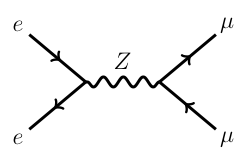
\includegraphics[width=.3\textwidth]{HW6a.png}

Consider the following plot that combines data from the Stanford Linear Collider and the Large Electron--Positron Collider\footnote{\url{https://arxiv.org/abs/hep-ex/0509008}}:

\begin{center}
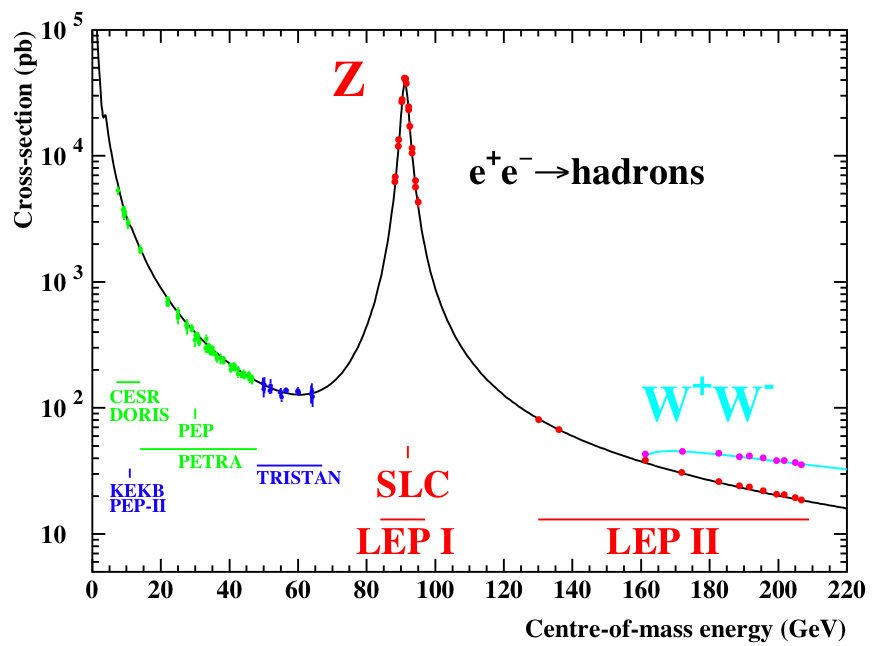
\includegraphics[width=.5\textwidth]{HW6aa.png}	
\end{center}

\begin{enumerate}
\item What is the mass of the $Z$ boson?
\item What is the order of magnitude of $\sqrt{M\Gamma}$? (\textsc{Hint}: the rate for a process goes like the amplitude times its complex conjugate.) \flip{2/14, added square root. Hint: $M^2\Gamma^2$ sets the width of the $Z$ peak. What's a good characteristic size for this width?}
\item What is the value of the $Z$ decay width in the PDG? (Full width.)
\item The decay width directly encodes the information of the $Z$ boson's lifetime. Based on your above answers and dimensional analysis, estimate the lifetime of the $Z$ boson. Answer in GeV to some power. 
\end{enumerate}


\end{document}